% Options for packages loaded elsewhere
\PassOptionsToPackage{unicode}{hyperref}
\PassOptionsToPackage{hyphens}{url}
%
\documentclass[
]{article}
\usepackage{amsmath,amssymb}
\usepackage{lmodern}
\usepackage{ifxetex,ifluatex}
\ifnum 0\ifxetex 1\fi\ifluatex 1\fi=0 % if pdftex
  \usepackage[T1]{fontenc}
  \usepackage[utf8]{inputenc}
  \usepackage{textcomp} % provide euro and other symbols
\else % if luatex or xetex
  \usepackage{unicode-math}
  \defaultfontfeatures{Scale=MatchLowercase}
  \defaultfontfeatures[\rmfamily]{Ligatures=TeX,Scale=1}
\fi
% Use upquote if available, for straight quotes in verbatim environments
\IfFileExists{upquote.sty}{\usepackage{upquote}}{}
\IfFileExists{microtype.sty}{% use microtype if available
  \usepackage[]{microtype}
  \UseMicrotypeSet[protrusion]{basicmath} % disable protrusion for tt fonts
}{}
\makeatletter
\@ifundefined{KOMAClassName}{% if non-KOMA class
  \IfFileExists{parskip.sty}{%
    \usepackage{parskip}
  }{% else
    \setlength{\parindent}{0pt}
    \setlength{\parskip}{6pt plus 2pt minus 1pt}}
}{% if KOMA class
  \KOMAoptions{parskip=half}}
\makeatother
\usepackage{xcolor}
\IfFileExists{xurl.sty}{\usepackage{xurl}}{} % add URL line breaks if available
\IfFileExists{bookmark.sty}{\usepackage{bookmark}}{\usepackage{hyperref}}
\hypersetup{
  pdftitle={MATH 4322 Homework 2 Solutions},
  pdfauthor={Instructor: Dr.~Cathy Poliak},
  hidelinks,
  pdfcreator={LaTeX via pandoc}}
\urlstyle{same} % disable monospaced font for URLs
\usepackage[margin=1in]{geometry}
\usepackage{color}
\usepackage{fancyvrb}
\newcommand{\VerbBar}{|}
\newcommand{\VERB}{\Verb[commandchars=\\\{\}]}
\DefineVerbatimEnvironment{Highlighting}{Verbatim}{commandchars=\\\{\}}
% Add ',fontsize=\small' for more characters per line
\usepackage{framed}
\definecolor{shadecolor}{RGB}{248,248,248}
\newenvironment{Shaded}{\begin{snugshade}}{\end{snugshade}}
\newcommand{\AlertTok}[1]{\textcolor[rgb]{0.94,0.16,0.16}{#1}}
\newcommand{\AnnotationTok}[1]{\textcolor[rgb]{0.56,0.35,0.01}{\textbf{\textit{#1}}}}
\newcommand{\AttributeTok}[1]{\textcolor[rgb]{0.77,0.63,0.00}{#1}}
\newcommand{\BaseNTok}[1]{\textcolor[rgb]{0.00,0.00,0.81}{#1}}
\newcommand{\BuiltInTok}[1]{#1}
\newcommand{\CharTok}[1]{\textcolor[rgb]{0.31,0.60,0.02}{#1}}
\newcommand{\CommentTok}[1]{\textcolor[rgb]{0.56,0.35,0.01}{\textit{#1}}}
\newcommand{\CommentVarTok}[1]{\textcolor[rgb]{0.56,0.35,0.01}{\textbf{\textit{#1}}}}
\newcommand{\ConstantTok}[1]{\textcolor[rgb]{0.00,0.00,0.00}{#1}}
\newcommand{\ControlFlowTok}[1]{\textcolor[rgb]{0.13,0.29,0.53}{\textbf{#1}}}
\newcommand{\DataTypeTok}[1]{\textcolor[rgb]{0.13,0.29,0.53}{#1}}
\newcommand{\DecValTok}[1]{\textcolor[rgb]{0.00,0.00,0.81}{#1}}
\newcommand{\DocumentationTok}[1]{\textcolor[rgb]{0.56,0.35,0.01}{\textbf{\textit{#1}}}}
\newcommand{\ErrorTok}[1]{\textcolor[rgb]{0.64,0.00,0.00}{\textbf{#1}}}
\newcommand{\ExtensionTok}[1]{#1}
\newcommand{\FloatTok}[1]{\textcolor[rgb]{0.00,0.00,0.81}{#1}}
\newcommand{\FunctionTok}[1]{\textcolor[rgb]{0.00,0.00,0.00}{#1}}
\newcommand{\ImportTok}[1]{#1}
\newcommand{\InformationTok}[1]{\textcolor[rgb]{0.56,0.35,0.01}{\textbf{\textit{#1}}}}
\newcommand{\KeywordTok}[1]{\textcolor[rgb]{0.13,0.29,0.53}{\textbf{#1}}}
\newcommand{\NormalTok}[1]{#1}
\newcommand{\OperatorTok}[1]{\textcolor[rgb]{0.81,0.36,0.00}{\textbf{#1}}}
\newcommand{\OtherTok}[1]{\textcolor[rgb]{0.56,0.35,0.01}{#1}}
\newcommand{\PreprocessorTok}[1]{\textcolor[rgb]{0.56,0.35,0.01}{\textit{#1}}}
\newcommand{\RegionMarkerTok}[1]{#1}
\newcommand{\SpecialCharTok}[1]{\textcolor[rgb]{0.00,0.00,0.00}{#1}}
\newcommand{\SpecialStringTok}[1]{\textcolor[rgb]{0.31,0.60,0.02}{#1}}
\newcommand{\StringTok}[1]{\textcolor[rgb]{0.31,0.60,0.02}{#1}}
\newcommand{\VariableTok}[1]{\textcolor[rgb]{0.00,0.00,0.00}{#1}}
\newcommand{\VerbatimStringTok}[1]{\textcolor[rgb]{0.31,0.60,0.02}{#1}}
\newcommand{\WarningTok}[1]{\textcolor[rgb]{0.56,0.35,0.01}{\textbf{\textit{#1}}}}
\usepackage{graphicx}
\makeatletter
\def\maxwidth{\ifdim\Gin@nat@width>\linewidth\linewidth\else\Gin@nat@width\fi}
\def\maxheight{\ifdim\Gin@nat@height>\textheight\textheight\else\Gin@nat@height\fi}
\makeatother
% Scale images if necessary, so that they will not overflow the page
% margins by default, and it is still possible to overwrite the defaults
% using explicit options in \includegraphics[width, height, ...]{}
\setkeys{Gin}{width=\maxwidth,height=\maxheight,keepaspectratio}
% Set default figure placement to htbp
\makeatletter
\def\fps@figure{htbp}
\makeatother
\setlength{\emergencystretch}{3em} % prevent overfull lines
\providecommand{\tightlist}{%
  \setlength{\itemsep}{0pt}\setlength{\parskip}{0pt}}
\setcounter{secnumdepth}{-\maxdimen} % remove section numbering
\ifluatex
  \usepackage{selnolig}  % disable illegal ligatures
\fi

\title{MATH 4322 Homework 2 Solutions}
\author{Instructor: Dr.~Cathy Poliak}
\date{9/24/2021}

\begin{document}
\maketitle

\hypertarget{problem-1}{%
\subsection{Problem 1}\label{problem-1}}

Suppose we have a data set with five predictors, \(X_1\) =GPA, \(X_2\) =
IQ, \(X_3\) = Gender (1 for Female and 0 for Male), \(X_4\) =
Interaction between GPA and IQ, and \(X_5\) = Interaction between GPA
and Gender. The response is starting salary after graduation (in
thousands of dollars). Suppose we use least squares to fit the model,
and get \(\hat{\beta}_0 = 50\), \(\hat{\beta}_1 = 20\),
\(\hat{\beta}_2= 0.07\),
\(\hat{\beta}_3 = 35\),\(\hat{\beta}_4 = 0.01\),
\(\hat{\beta}_5 = -10\).

\begin{enumerate}
\def\labelenumi{(\alph{enumi})}
\tightlist
\item
  Which answer is correct, and why?

  \begin{enumerate}
  \def\labelenumii{\roman{enumii}.}
  \setcounter{enumii}{2}
  \tightlist
  \item
    For a fixed value of IQ and GPA, males earn more on average than
    females provided that the GPA is high enough because:
  \end{enumerate}
\end{enumerate}

\begin{itemize}
\tightlist
\item
  The predicted regression equation for multiple variables is:

  \begin{itemize}
  \tightlist
  \item
    \(\hat{Y} = 50 + 20X_1 + 0.07X_2 + 35X_3 + 0.01X_4 - 10X_5\)\\
  \end{itemize}
\item
  The male regression equation is:

  \begin{itemize}
  \tightlist
  \item
    \(\hat{Y}_m = 50 + 20X_1 + 0.07X_2 + 0.01X_4\)\\
  \end{itemize}
\item
  The female regression equation is:

  \begin{itemize}
  \tightlist
  \item
    \(\hat{Y}_f = 85 + 20X_1 + 0.07X_2 + 0.01X_4 - 10X_5\)
  \end{itemize}
\end{itemize}

\begin{enumerate}
\def\labelenumi{(\alph{enumi})}
\setcounter{enumi}{1}
\tightlist
\item
  Predict the salary of a female with IQ of 110 and a GPA of 4.0.
\end{enumerate}

\begin{itemize}
\tightlist
\item
  \(\hat{Y}_f = 85 + 20X_1 + 0.07X_2 + 0.01X_4 - 10X_5\)
\item
  \(\hat{Y}_f = 85 + 20(4.0) + 0.07(110) + 0.1(4 * 110) - 10(4 * 1)\)
\end{itemize}

\begin{Shaded}
\begin{Highlighting}[]
\NormalTok{(}\AttributeTok{Y\_f =} \DecValTok{85} \SpecialCharTok{+} \DecValTok{20}\SpecialCharTok{*}\NormalTok{(}\FloatTok{4.0}\NormalTok{) }\SpecialCharTok{+} \FloatTok{0.07}\SpecialCharTok{*}\NormalTok{(}\DecValTok{110}\NormalTok{) }\SpecialCharTok{+} \FloatTok{0.01}\SpecialCharTok{*}\NormalTok{(}\DecValTok{4} \SpecialCharTok{*} \DecValTok{110}\NormalTok{) }\SpecialCharTok{{-}} \DecValTok{10}\SpecialCharTok{*}\NormalTok{(}\DecValTok{4} \SpecialCharTok{*} \DecValTok{1}\NormalTok{))}
\end{Highlighting}
\end{Shaded}

\begin{verbatim}
## [1] 137.1
\end{verbatim}

\begin{enumerate}
\def\labelenumi{(\alph{enumi})}
\setcounter{enumi}{2}
\tightlist
\item
  True or false: Since the coefficient for the GPA/IQ interaction term
  is very small, there is very little evidence of an interaction effect.
  Justify your answer.
\end{enumerate}

\begin{itemize}
\tightlist
\item
  \textbf{False}, because it also depends on the \(SE\) of the \(beta\)
  estimator
\end{itemize}

\hypertarget{problem-2}{%
\subsection{Problem 2}\label{problem-2}}

We perform stepwise, forward stepwise, and backward stepwise selection
on a single data set. For each approach, we obtain \(p + 1\) models,
containing \(0, 1, 2, \ldots , p\) predictors. True or False:

\begin{enumerate}
\def\labelenumi{(\alph{enumi})}
\tightlist
\item
  The predictors in the \(k\)-variable model identified by forward
  stepwise are a subset of the predictors in the (\(k+1\))-variable
  model identified by forward stepwise selection.
\end{enumerate}

\begin{itemize}
\tightlist
\item
  \textbf{True}, because in forward selection each predictors is added
  at each step. \(k+1)\) variables are considered as predictors for the
  model.
\end{itemize}

\begin{enumerate}
\def\labelenumi{(\alph{enumi})}
\setcounter{enumi}{1}
\tightlist
\item
  The predictors in the \(k\)-variable model identified by backward
  stepwise are a subset of the predictors in the (\(k + 1\))-variable
  model identified by backward stepwise selection.
\end{enumerate}

\begin{itemize}
\tightlist
\item
  \textbf{True}, by testing if any variable in test effective then those
  variable will be affected. The model will remain with \(k\) variables
  in next step.
\end{itemize}

\begin{enumerate}
\def\labelenumi{(\alph{enumi})}
\setcounter{enumi}{2}
\tightlist
\item
  The predictors in the \(k\)-variable model identified by backward
  stepwise are a subset of the predictors in the (\(k + 1\))-variable
  model identified by forward stepwise selection.
\end{enumerate}

\begin{itemize}
\tightlist
\item
  \textbf{False}, the predictors of model with \(k + 1\) variables from
  backward selection method are form by deleting each term after
  checking the less effective variable and deleting them.
\end{itemize}

\begin{enumerate}
\def\labelenumi{(\alph{enumi})}
\setcounter{enumi}{3}
\tightlist
\item
  The predictors in the \(k\)-variable model identified by forward
  stepwise are a subset of the predictors in the (\(k+1\))-variable
  model identified by backward stepwise selection.
\end{enumerate}

\begin{itemize}
\tightlist
\item
  \textbf{False}, the \(k\) variables in the predictor model by backward
  selection method and cannot be subset of \(k+1\) variables in the
  model by foward selection because they're different
\end{itemize}

\begin{enumerate}
\def\labelenumi{(\alph{enumi})}
\setcounter{enumi}{4}
\tightlist
\item
  The predictors in the \(k\)-variable model identified by stepwise are
  a subset of the predictors in the (\(k + 1\))-variable model
  identified by stepwise selection.
\end{enumerate}

\begin{itemize}
\tightlist
\item
  \textbf{True}, the predictors in the \(k\) variable model identified
  by best subset are subset of the predictors in the \(k+1\) variable
  model.
\end{itemize}

\newpage

\hypertarget{problem-3}{%
\subsection{Problem 3}\label{problem-3}}

This question involves the use of simple linear regression on the
\emph{Auto} data set.

\begin{enumerate}
\def\labelenumi{(\alph{enumi})}
\tightlist
\item
  Use the \texttt{lm()} function to perform a simple linear regression
  with \emph{mpg} as the response and \emph{horsepower} (\emph{hp}) as
  the predictor. Use the \texttt{summary()} function to print the
  results. Comment on the output. For example:
\end{enumerate}

\begin{Shaded}
\begin{Highlighting}[]
\FunctionTok{library}\NormalTok{(ISLR)}
\FunctionTok{attach}\NormalTok{(Auto)}
\NormalTok{mpg\_horsepower }\OtherTok{=} \FunctionTok{lm}\NormalTok{(mpg }\SpecialCharTok{\textasciitilde{}}\NormalTok{ horsepower)}
\FunctionTok{summary}\NormalTok{(mpg\_horsepower)}
\end{Highlighting}
\end{Shaded}

\begin{verbatim}
## 
## Call:
## lm(formula = mpg ~ horsepower)
## 
## Residuals:
##      Min       1Q   Median       3Q      Max 
## -13.5710  -3.2592  -0.3435   2.7630  16.9240 
## 
## Coefficients:
##              Estimate Std. Error t value Pr(>|t|)    
## (Intercept) 39.935861   0.717499   55.66   <2e-16 ***
## horsepower  -0.157845   0.006446  -24.49   <2e-16 ***
## ---
## Signif. codes:  0 '***' 0.001 '**' 0.01 '*' 0.05 '.' 0.1 ' ' 1
## 
## Residual standard error: 4.906 on 390 degrees of freedom
## Multiple R-squared:  0.6059, Adjusted R-squared:  0.6049 
## F-statistic: 599.7 on 1 and 390 DF,  p-value: < 2.2e-16
\end{verbatim}

\begin{itemize}
\item
  \begin{enumerate}
  \def\labelenumi{\roman{enumi}.}
  \tightlist
  \item
    Is there a relationship between the predictor and the response?
  \end{enumerate}

  \begin{itemize}
  \tightlist
  \item
    Yes, there is a relationship between the predictor and the response,
    the \(p-value = 2e-16 = 0 < {a = 0.05}\)
  \end{itemize}
\item
  \begin{enumerate}
  \def\labelenumi{\roman{enumi}.}
  \setcounter{enumi}{1}
  \tightlist
  \item
    How strong is the relationship between the predictor and the
    response?
  \end{enumerate}
\end{itemize}

\begin{Shaded}
\begin{Highlighting}[]
\FunctionTok{cor}\NormalTok{(mpg, horsepower)}
\end{Highlighting}
\end{Shaded}

\begin{verbatim}
## [1] -0.7784268
\end{verbatim}

\begin{itemize}
\item
  \begin{enumerate}
  \def\labelenumi{\roman{enumi}.}
  \setcounter{enumi}{2}
  \tightlist
  \item
    Is the relationship between the predictor and the response positive
    or negative?
  \end{enumerate}

  \begin{itemize}
  \tightlist
  \item
    The relationship between the predictor and the response is negative,
    because it have a negative correlation.
  \end{itemize}
\item
  \begin{enumerate}
  \def\labelenumi{\roman{enumi}.}
  \setcounter{enumi}{3}
  \tightlist
  \item
    What is the predicted mpg associated with a horsepower of 98? What
    are the associated 95\% confidence and prediction intervals? Give an
    interpretation of these intervals.
  \end{enumerate}

  \begin{itemize}
  \tightlist
  \item
    \(Y = 39.935 - 0.1578X\)
  \item
    The predicted \emph{mpg} associated with a \emph{horsepower} of 98
    is:
  \end{itemize}
\end{itemize}

\begin{Shaded}
\begin{Highlighting}[]
\NormalTok{(}\AttributeTok{Y =} \FloatTok{39.935} \SpecialCharTok{{-}} \FloatTok{0.1578} \SpecialCharTok{*} \DecValTok{98}\NormalTok{)}
\end{Highlighting}
\end{Shaded}

\begin{verbatim}
## [1] 24.4706
\end{verbatim}

\begin{itemize}
\tightlist
\item
  The \emph{predict interval} is:
\end{itemize}

\begin{Shaded}
\begin{Highlighting}[]
\NormalTok{horsedata }\OtherTok{=} \FunctionTok{data.frame}\NormalTok{(}\AttributeTok{horsepower =} \DecValTok{98}\NormalTok{)}
\CommentTok{\#for predict}
\FunctionTok{predict}\NormalTok{(mpg\_horsepower, horsedata, }\AttributeTok{interval =} \StringTok{"predict"}\NormalTok{)}
\end{Highlighting}
\end{Shaded}

\begin{verbatim}
##        fit     lwr      upr
## 1 24.46708 14.8094 34.12476
\end{verbatim}

\begin{itemize}
\item
  This means the predicted \emph{mpg} for a \(horsepower = 98\) is
  between \([14.80, 34.12]\) with a \(95\%\) confidence
\item
  The \emph{confidence interval} is:
\end{itemize}

\begin{Shaded}
\begin{Highlighting}[]
\CommentTok{\#for confidence}
\FunctionTok{predict}\NormalTok{(mpg\_horsepower, horsedata, }\AttributeTok{interval =} \StringTok{"confidence"}\NormalTok{)}
\end{Highlighting}
\end{Shaded}

\begin{verbatim}
##        fit      lwr      upr
## 1 24.46708 23.97308 24.96108
\end{verbatim}

\begin{itemize}
\tightlist
\item
  This means we predict the \textbf{average} \emph{mpg} with
  \(horsepower = 98\) is between \([23.97, 24.96]\) with \(95\%\)
  confidence.
\end{itemize}

\begin{enumerate}
\def\labelenumi{(\alph{enumi})}
\setcounter{enumi}{1}
\tightlist
\item
  Plot the response and the predictor. Use the \texttt{abline()}
  function to display the least squares regression line.
\end{enumerate}

\begin{Shaded}
\begin{Highlighting}[]
\FunctionTok{plot}\NormalTok{(mpg}\SpecialCharTok{\textasciitilde{}}\NormalTok{horsepower, }\AttributeTok{pch=}\DecValTok{16}\NormalTok{)}
\FunctionTok{abline}\NormalTok{(mpg\_horsepower, }\AttributeTok{col =} \StringTok{"red"}\NormalTok{)}
\end{Highlighting}
\end{Shaded}

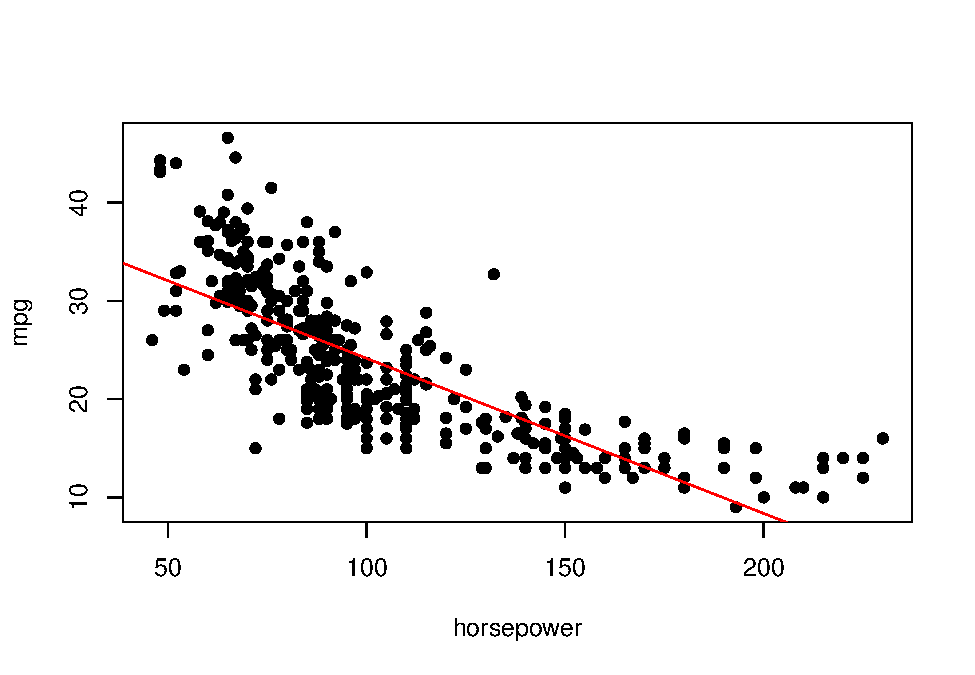
\includegraphics{math4322_fall21_hw2_files/figure-latex/unnamed-chunk-7-1.pdf}
(c) Use the \texttt{plot()} function to produce diagnostic plots of the
least squares regression fit. Comment on any problems you see with the
fit.

\begin{Shaded}
\begin{Highlighting}[]
\FunctionTok{par}\NormalTok{(}\AttributeTok{mfrow =} \FunctionTok{c}\NormalTok{(}\DecValTok{2}\NormalTok{,}\DecValTok{2}\NormalTok{))}
\FunctionTok{plot}\NormalTok{(mpg\_horsepower)}
\end{Highlighting}
\end{Shaded}

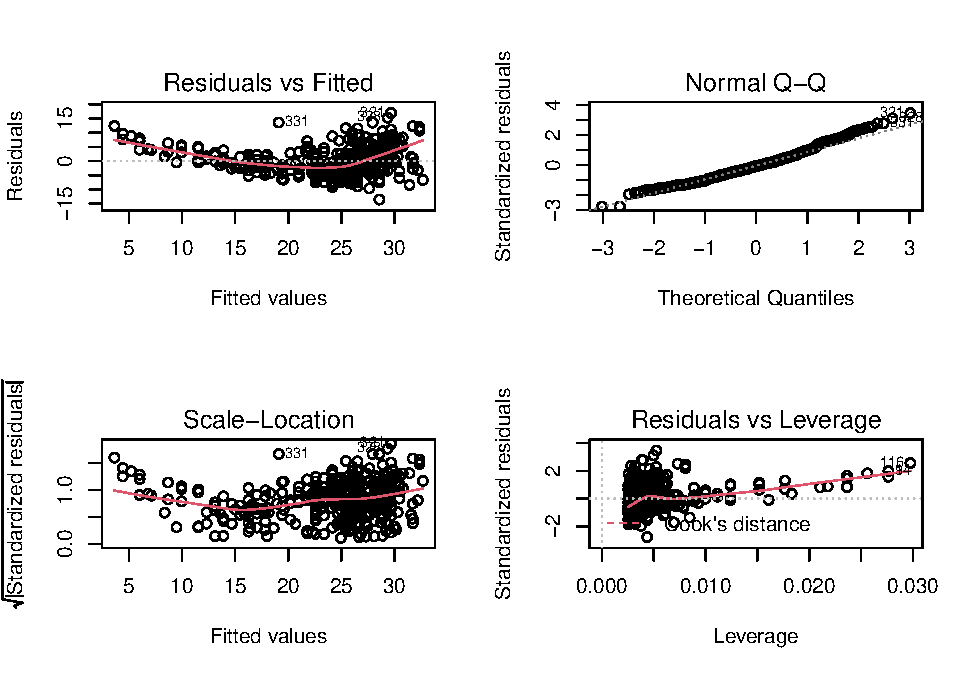
\includegraphics{math4322_fall21_hw2_files/figure-latex/unnamed-chunk-8-1.pdf}
* These plot show some outliers observation numbers: 321, 331, 328\\
* High leverage: 116, 94\\
* It appears that the linearity fit is a little curvy

\hypertarget{problem-4}{%
\subsection{Problem 4}\label{problem-4}}

This question involves the use of multiple linear regression on the
\emph{Auto} data set.

\begin{enumerate}
\def\labelenumi{(\alph{enumi})}
\tightlist
\item
  Produce a scatterplot matrix which includes all of the variables in
  the data set.
\end{enumerate}

\begin{Shaded}
\begin{Highlighting}[]
\FunctionTok{head}\NormalTok{(Auto)}
\end{Highlighting}
\end{Shaded}

\begin{verbatim}
##   mpg cylinders displacement horsepower weight acceleration year origin
## 1  18         8          307        130   3504         12.0   70      1
## 2  15         8          350        165   3693         11.5   70      1
## 3  18         8          318        150   3436         11.0   70      1
## 4  16         8          304        150   3433         12.0   70      1
## 5  17         8          302        140   3449         10.5   70      1
## 6  15         8          429        198   4341         10.0   70      1
##                        name
## 1 chevrolet chevelle malibu
## 2         buick skylark 320
## 3        plymouth satellite
## 4             amc rebel sst
## 5               ford torino
## 6          ford galaxie 500
\end{verbatim}

\begin{Shaded}
\begin{Highlighting}[]
\FunctionTok{plot}\NormalTok{(Auto)}
\end{Highlighting}
\end{Shaded}

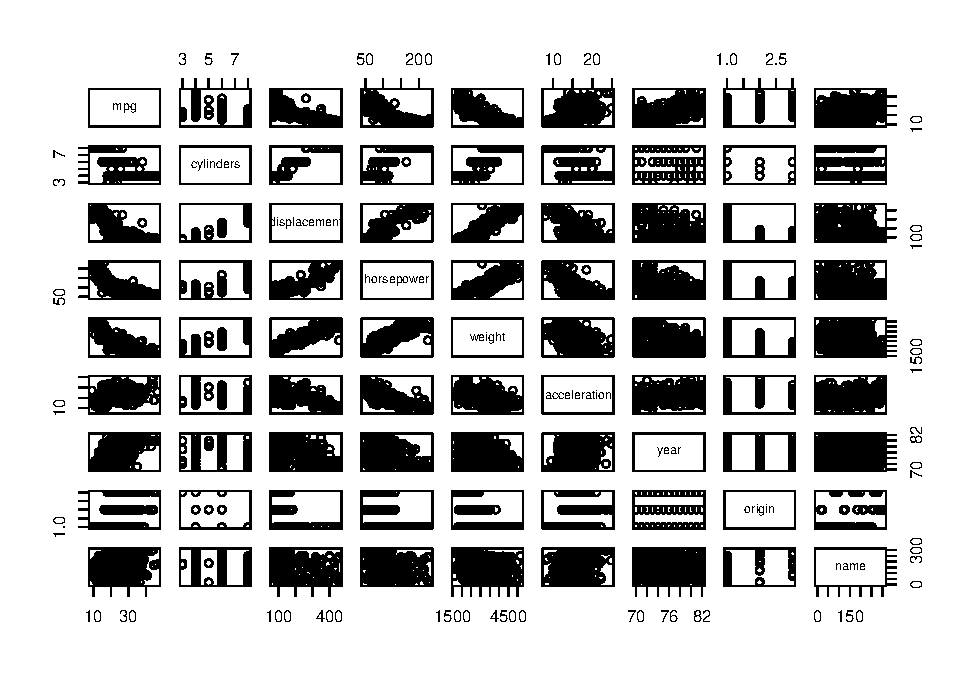
\includegraphics{math4322_fall21_hw2_files/figure-latex/unnamed-chunk-9-1.pdf}
(b) Compute the matrix of correlations between the variables using the
function \texttt{cor()}. You will need to exclude the name variable,
\texttt{cor()} which is qualitative.

\begin{Shaded}
\begin{Highlighting}[]
\NormalTok{?Auto}
\CommentTok{\#9 variables}
\NormalTok{(}\AttributeTok{correlation =} \FunctionTok{cor}\NormalTok{(Auto[,}\SpecialCharTok{{-}}\DecValTok{9}\NormalTok{]))}
\end{Highlighting}
\end{Shaded}

\begin{verbatim}
##                     mpg  cylinders displacement horsepower     weight
## mpg           1.0000000 -0.7776175   -0.8051269 -0.7784268 -0.8322442
## cylinders    -0.7776175  1.0000000    0.9508233  0.8429834  0.8975273
## displacement -0.8051269  0.9508233    1.0000000  0.8972570  0.9329944
## horsepower   -0.7784268  0.8429834    0.8972570  1.0000000  0.8645377
## weight       -0.8322442  0.8975273    0.9329944  0.8645377  1.0000000
## acceleration  0.4233285 -0.5046834   -0.5438005 -0.6891955 -0.4168392
## year          0.5805410 -0.3456474   -0.3698552 -0.4163615 -0.3091199
## origin        0.5652088 -0.5689316   -0.6145351 -0.4551715 -0.5850054
##              acceleration       year     origin
## mpg             0.4233285  0.5805410  0.5652088
## cylinders      -0.5046834 -0.3456474 -0.5689316
## displacement   -0.5438005 -0.3698552 -0.6145351
## horsepower     -0.6891955 -0.4163615 -0.4551715
## weight         -0.4168392 -0.3091199 -0.5850054
## acceleration    1.0000000  0.2903161  0.2127458
## year            0.2903161  1.0000000  0.1815277
## origin          0.2127458  0.1815277  1.0000000
\end{verbatim}

\begin{enumerate}
\def\labelenumi{(\alph{enumi})}
\setcounter{enumi}{2}
\tightlist
\item
  Use the \texttt{lm()} function to perform a multiple linear regression
  with \emph{mpg} as the response and all other variables except name as
  the predictors. Use the \texttt{summary()} function to print the
  results. Comment on the output. For instance:
\end{enumerate}

\begin{Shaded}
\begin{Highlighting}[]
\NormalTok{auto.new }\OtherTok{=}\NormalTok{ Auto[, }\SpecialCharTok{{-}}\DecValTok{9}\NormalTok{] }\CommentTok{\#8 variables}
\NormalTok{auto.new}\SpecialCharTok{$}\NormalTok{origin }\OtherTok{=} \FunctionTok{as.factor}\NormalTok{(auto.new}\SpecialCharTok{$}\NormalTok{origin) }\CommentTok{\#set to factor}
\NormalTok{auto.new}\SpecialCharTok{$}\NormalTok{cylinders }\OtherTok{=} \FunctionTok{as.factor}\NormalTok{(auto.new}\SpecialCharTok{$}\NormalTok{cylinders)}
\NormalTok{auto.lm }\OtherTok{=} \FunctionTok{lm}\NormalTok{(mpg}\SpecialCharTok{\textasciitilde{}}\NormalTok{., }\AttributeTok{data =}\NormalTok{ auto.new)  }\CommentTok{\#linear model}
\FunctionTok{summary}\NormalTok{(auto.lm)}
\end{Highlighting}
\end{Shaded}

\begin{verbatim}
## 
## Call:
## lm(formula = mpg ~ ., data = auto.new)
## 
## Residuals:
##     Min      1Q  Median      3Q     Max 
## -8.6797 -1.9373 -0.0678  1.6711 12.7756 
## 
## Coefficients:
##                Estimate Std. Error t value Pr(>|t|)    
## (Intercept)  -2.208e+01  4.541e+00  -4.862 1.70e-06 ***
## cylinders4    6.722e+00  1.654e+00   4.064 5.85e-05 ***
## cylinders5    7.078e+00  2.516e+00   2.813  0.00516 ** 
## cylinders6    3.351e+00  1.824e+00   1.837  0.06701 .  
## cylinders8    5.099e+00  2.109e+00   2.418  0.01607 *  
## displacement  1.870e-02  7.222e-03   2.590  0.00997 ** 
## horsepower   -3.490e-02  1.323e-02  -2.639  0.00866 ** 
## weight       -5.780e-03  6.315e-04  -9.154  < 2e-16 ***
## acceleration  2.598e-02  9.304e-02   0.279  0.78021    
## year          7.370e-01  4.892e-02  15.064  < 2e-16 ***
## origin2       1.764e+00  5.513e-01   3.200  0.00149 ** 
## origin3       2.617e+00  5.272e-01   4.964 1.04e-06 ***
## ---
## Signif. codes:  0 '***' 0.001 '**' 0.01 '*' 0.05 '.' 0.1 ' ' 1
## 
## Residual standard error: 3.098 on 380 degrees of freedom
## Multiple R-squared:  0.8469, Adjusted R-squared:  0.8425 
## F-statistic: 191.1 on 11 and 380 DF,  p-value: < 2.2e-16
\end{verbatim}

\begin{enumerate}
\def\labelenumi{\roman{enumi}.}
\tightlist
\item
  Is there a relationship between the predictors and the response?
\end{enumerate}

\begin{itemize}
\tightlist
\item
  \(p-value = 2.2e-16 < a = 0.05\), therefore there is a relationship
  between the predictors and the response.
\end{itemize}

\begin{enumerate}
\def\labelenumi{\roman{enumi}.}
\setcounter{enumi}{1}
\tightlist
\item
  Which predictors appear to have a statistically significant
  relationship to the response?
\end{enumerate}

\begin{itemize}
\tightlist
\item
  The predictors that appear to have a statistically significant
  relationship to the response is \emph{cylinders4, cylinders5,
  cylinders6, cylinders8, displacement, horsepower, weight, year,
  origin2 and origin3\$}, because their \(p-value\) is significant.
\end{itemize}

\begin{enumerate}
\def\labelenumi{\roman{enumi}.}
\setcounter{enumi}{2}
\tightlist
\item
  What does the coefficient for the year variable suggest?
\end{enumerate}

\begin{itemize}
\tightlist
\item
  For testing each one predictor separately , \(H_0 : B_j = 0\) it
  appears that only \emph{acceleration} does not have a statistically
  significant to \emph{mpg}
\end{itemize}

\begin{enumerate}
\def\labelenumi{(\alph{enumi})}
\setcounter{enumi}{3}
\tightlist
\item
  Use the \texttt{plot()} function to produce diagnostic plots of the
  linear regression fit based on the predictors that appear to have a
  statistically signifianct relationship to the response. Comment on any
  problems you see with the fit. Do the residual plots suggest any
  unusually large outliers? Does the leverage plot identify any
  observations with unusually high leverage?
\end{enumerate}

\begin{Shaded}
\begin{Highlighting}[]
\NormalTok{auto.new2 }\OtherTok{=}\NormalTok{ auto.new[, }\SpecialCharTok{{-}}\DecValTok{6}\NormalTok{] }\CommentTok{\#take out the 6th variable in auto.new}
\NormalTok{auto.lm2 }\OtherTok{=} \FunctionTok{lm}\NormalTok{(mpg}\SpecialCharTok{\textasciitilde{}}\NormalTok{., }\AttributeTok{data =}\NormalTok{ auto.new2) }\CommentTok{\#linear model2}
\FunctionTok{summary}\NormalTok{(auto.lm2)}
\end{Highlighting}
\end{Shaded}

\begin{verbatim}
## 
## Call:
## lm(formula = mpg ~ ., data = auto.new2)
## 
## Residuals:
##     Min      1Q  Median      3Q     Max 
## -8.7037 -1.9501 -0.0552  1.7105 12.7932 
## 
## Coefficients:
##                Estimate Std. Error t value Pr(>|t|)    
## (Intercept)  -2.162e+01  4.231e+00  -5.111 5.09e-07 ***
## cylinders4    6.784e+00  1.637e+00   4.144 4.20e-05 ***
## cylinders5    7.147e+00  2.501e+00   2.857 0.004510 ** 
## cylinders6    3.403e+00  1.813e+00   1.877 0.061262 .  
## cylinders8    5.137e+00  2.102e+00   2.444 0.014983 *  
## displacement  1.848e-02  7.169e-03   2.578 0.010312 *  
## horsepower   -3.706e-02  1.071e-02  -3.459 0.000604 ***
## weight       -5.696e-03  5.535e-04 -10.291  < 2e-16 ***
## year          7.358e-01  4.868e-02  15.114  < 2e-16 ***
## origin2       1.763e+00  5.506e-01   3.203 0.001476 ** 
## origin3       2.621e+00  5.264e-01   4.979 9.71e-07 ***
## ---
## Signif. codes:  0 '***' 0.001 '**' 0.01 '*' 0.05 '.' 0.1 ' ' 1
## 
## Residual standard error: 3.094 on 381 degrees of freedom
## Multiple R-squared:  0.8469, Adjusted R-squared:  0.8429 
## F-statistic: 210.7 on 10 and 381 DF,  p-value: < 2.2e-16
\end{verbatim}

\begin{Shaded}
\begin{Highlighting}[]
\FunctionTok{par}\NormalTok{(}\AttributeTok{mfrow =} \FunctionTok{c}\NormalTok{(}\DecValTok{2}\NormalTok{,}\DecValTok{2}\NormalTok{))}
\FunctionTok{plot}\NormalTok{(auto.lm2)}
\end{Highlighting}
\end{Shaded}

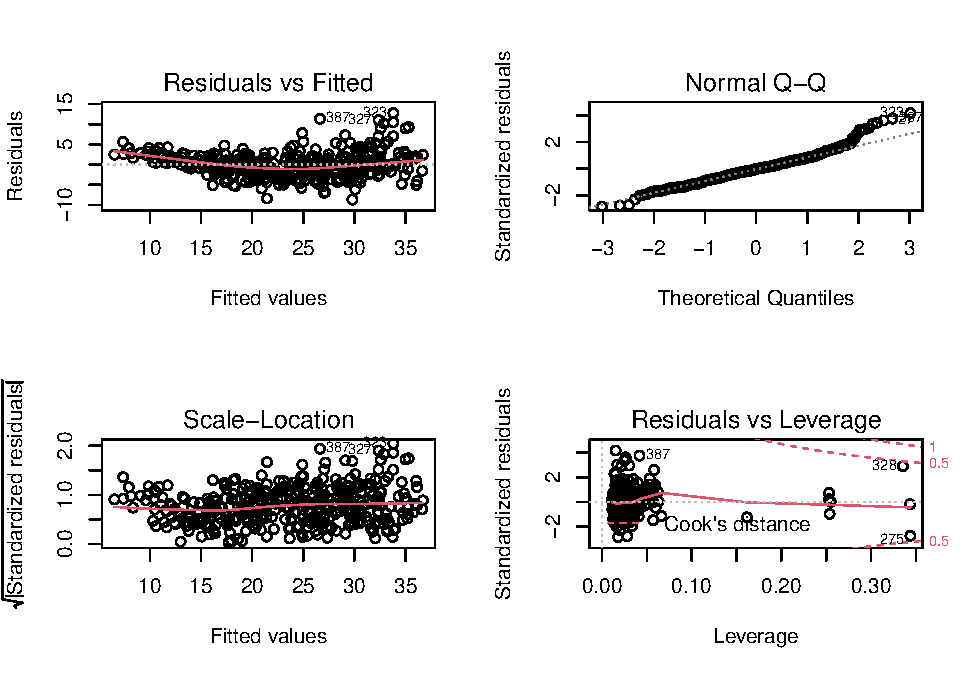
\includegraphics{math4322_fall21_hw2_files/figure-latex/unnamed-chunk-13-1.pdf}
* These plots show some outliers observation numbers: 387, 323, 327\\
* High leverage: 387, 328, 275\\
* It appears that the linearity fit is good.\\
(e) Use the * and/or : symbols to fit linear regression models with
interaction effects. Do any interactions appear to be statistically
significant?

\begin{Shaded}
\begin{Highlighting}[]
\CommentTok{\#interactiion model between displacment: horsepower and horsepower: weight}
\NormalTok{auto.int }\OtherTok{=} \FunctionTok{lm}\NormalTok{(mpg }\SpecialCharTok{\textasciitilde{}}\NormalTok{ cylinders }\SpecialCharTok{+}\NormalTok{ displacement }\SpecialCharTok{*}\NormalTok{ horsepower }\SpecialCharTok{+}\NormalTok{ horsepower}\SpecialCharTok{*}\NormalTok{weight }\SpecialCharTok{+}\NormalTok{ year }\SpecialCharTok{+}\NormalTok{ origin, }\AttributeTok{data =}\NormalTok{ auto.new2)}
\FunctionTok{summary}\NormalTok{(auto.int)}
\end{Highlighting}
\end{Shaded}

\begin{verbatim}
## 
## Call:
## lm(formula = mpg ~ cylinders + displacement * horsepower + horsepower * 
##     weight + year + origin, data = auto.new2)
## 
## Residuals:
##     Min      1Q  Median      3Q     Max 
## -6.7565 -1.4899 -0.0843  1.4168 12.0178 
## 
## Coefficients:
##                           Estimate Std. Error t value Pr(>|t|)    
## (Intercept)             -7.583e+00  4.316e+00  -1.757 0.079734 .  
## cylinders4               5.856e+00  1.516e+00   3.863 0.000132 ***
## cylinders5               7.464e+00  2.297e+00   3.250 0.001259 ** 
## cylinders6               5.197e+00  1.728e+00   3.008 0.002803 ** 
## cylinders8               6.455e+00  2.042e+00   3.161 0.001700 ** 
## displacement            -2.243e-02  1.660e-02  -1.351 0.177530    
## horsepower              -1.842e-01  2.162e-02  -8.521 3.79e-16 ***
## weight                  -7.717e-03  1.513e-03  -5.099 5.41e-07 ***
## year                     7.523e-01  4.523e-02  16.635  < 2e-16 ***
## origin2                  1.056e+00  5.251e-01   2.011 0.045084 *  
## origin3                  1.695e+00  4.971e-01   3.411 0.000718 ***
## displacement:horsepower  1.968e-04  9.529e-05   2.066 0.039544 *  
## horsepower:weight        2.768e-05  1.047e-05   2.644 0.008533 ** 
## ---
## Signif. codes:  0 '***' 0.001 '**' 0.01 '*' 0.05 '.' 0.1 ' ' 1
## 
## Residual standard error: 2.84 on 379 degrees of freedom
## Multiple R-squared:  0.8716, Adjusted R-squared:  0.8676 
## F-statistic: 214.4 on 12 and 379 DF,  p-value: < 2.2e-16
\end{verbatim}

\begin{itemize}
\tightlist
\item
  It appears that there might be interaction effects with horsepower and
  displacement also horsepower and weight. However, when we add these
  interaction terms, the displacement is no longer significant.
\end{itemize}

\begin{enumerate}
\def\labelenumi{(\alph{enumi})}
\setcounter{enumi}{5}
\tightlist
\item
  Try a few different transformations of the variables, such as
  \emph{log(X)}, \(\sqrt{X}\), \(X^2\). Comment on your findings.
\end{enumerate}

\begin{Shaded}
\begin{Highlighting}[]
\NormalTok{auto.lm3 }\OtherTok{=} \FunctionTok{lm}\NormalTok{(mpg }\SpecialCharTok{\textasciitilde{}}\NormalTok{ cylinders }\SpecialCharTok{+}\NormalTok{ displacement }\SpecialCharTok{+} \FunctionTok{sqrt}\NormalTok{(horsepower) }\SpecialCharTok{+}\NormalTok{ weight }\SpecialCharTok{+}\NormalTok{ origin, }\AttributeTok{data =}\NormalTok{ auto.new2)}
\FunctionTok{summary}\NormalTok{(auto.lm3)}
\end{Highlighting}
\end{Shaded}

\begin{verbatim}
## 
## Call:
## lm(formula = mpg ~ cylinders + displacement + sqrt(horsepower) + 
##     weight + origin, data = auto.new2)
## 
## Residuals:
##    Min     1Q Median     3Q    Max 
## -9.994 -2.235 -0.542  1.758 15.765 
## 
## Coefficients:
##                    Estimate Std. Error t value Pr(>|t|)    
## (Intercept)      44.0684287  3.1692690  13.905  < 2e-16 ***
## cylinders4        7.8227761  2.0337518   3.846  0.00014 ***
## cylinders5        9.9647779  3.0964663   3.218  0.00140 ** 
## cylinders6        4.0868709  2.2409849   1.824  0.06898 .  
## cylinders8        6.2616424  2.6039750   2.405  0.01666 *  
## displacement      0.0063803  0.0085501   0.746  0.45599    
## sqrt(horsepower) -1.7726717  0.2759663  -6.424 3.96e-10 ***
## weight           -0.0037309  0.0006861  -5.438 9.65e-08 ***
## origin2           0.0051860  0.6652473   0.008  0.99378    
## origin3           2.6162364  0.6490513   4.031 6.71e-05 ***
## ---
## Signif. codes:  0 '***' 0.001 '**' 0.01 '*' 0.05 '.' 0.1 ' ' 1
## 
## Residual standard error: 3.845 on 382 degrees of freedom
## Multiple R-squared:  0.7629, Adjusted R-squared:  0.7573 
## F-statistic: 136.6 on 9 and 382 DF,  p-value: < 2.2e-16
\end{verbatim}

\begin{itemize}
\tightlist
\item
  The adjusted R-squared actually got lower when i \(sqrt(horsepower)\)
  \newpage
\end{itemize}

\hypertarget{problem-5}{%
\subsection{Problem 5}\label{problem-5}}

This problem focuses on the \textbf{collinearity} problem.

\begin{enumerate}
\def\labelenumi{(\alph{enumi})}
\tightlist
\item
  Perform the following commands in R:
\end{enumerate}

\begin{Shaded}
\begin{Highlighting}[]
\FunctionTok{set.seed}\NormalTok{ (}\DecValTok{1}\NormalTok{)}
\NormalTok{x1}\OtherTok{=}\FunctionTok{runif}\NormalTok{ (}\DecValTok{100}\NormalTok{)}
\NormalTok{x2 }\OtherTok{=}\FloatTok{0.5}\SpecialCharTok{*}\NormalTok{ x1}\SpecialCharTok{+}\FunctionTok{rnorm}\NormalTok{ (}\DecValTok{100}\NormalTok{) }\SpecialCharTok{/}\DecValTok{10}
\NormalTok{y}\OtherTok{=}\DecValTok{2}\SpecialCharTok{+}\DecValTok{2}\SpecialCharTok{*}\NormalTok{ x1 }\SpecialCharTok{+}\FloatTok{0.3}\SpecialCharTok{*}\NormalTok{ x2}\SpecialCharTok{+}\FunctionTok{rnorm}\NormalTok{ (}\DecValTok{100}\NormalTok{)}
\end{Highlighting}
\end{Shaded}

The last line corresponds to creating a linear model in which \(y\) is a
function of \(x_1\) and \(x_2\). Write out the form of the linear model.
What are the regression coefficients?

\begin{enumerate}
\def\labelenumi{(\alph{enumi})}
\setcounter{enumi}{1}
\tightlist
\item
  What is the correlation between \(x_1\) and \(x_2\)? Create a
  scatterplot displaying the relationship between the variables.
\end{enumerate}

\begin{Shaded}
\begin{Highlighting}[]
\FunctionTok{cor}\NormalTok{(x1, x2)}
\end{Highlighting}
\end{Shaded}

\begin{verbatim}
## [1] 0.8351212
\end{verbatim}

\begin{Shaded}
\begin{Highlighting}[]
\FunctionTok{plot}\NormalTok{(x1, x2)}
\end{Highlighting}
\end{Shaded}

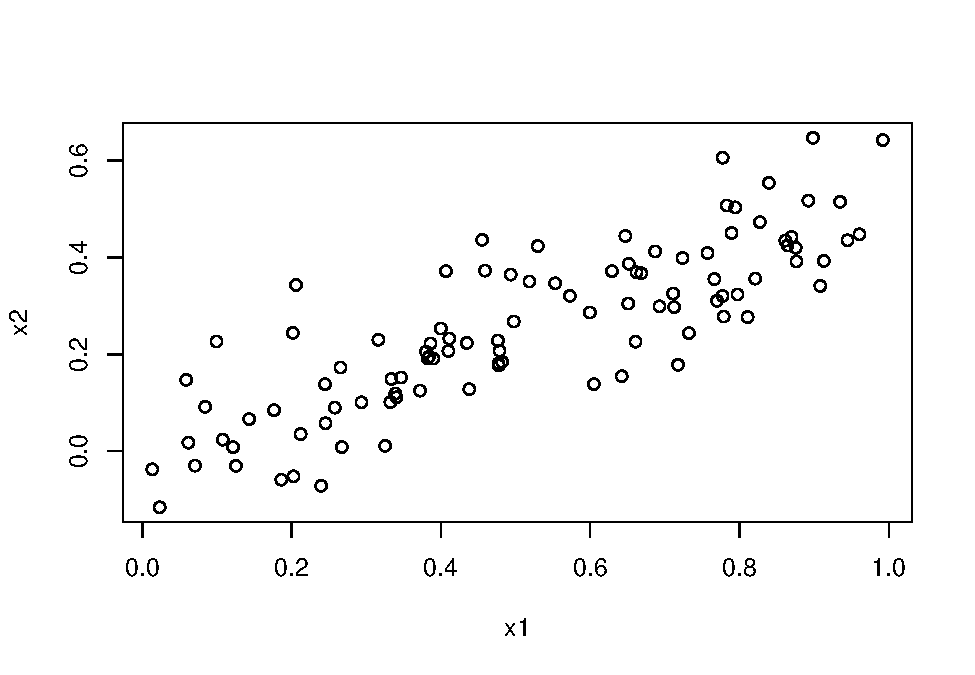
\includegraphics{math4322_fall21_hw2_files/figure-latex/unnamed-chunk-17-1.pdf}
(c) Using this data, fit a least squares regression to predict y using
\(x_1\) and \(x_2\). Describe the results obtained. What are
\(\hat{\beta}_0\), \(\hat{\beta}_1\), and \(\hat{\beta}_2\)? How do
these relate to the true \(\beta_0\), \(\beta_1\), and \(\beta_2\)? Can
you reject the null hypothesis \(H_0 : \beta_1 = 0\)? How about the null
hypothesis \(H_0 : \beta_2 = 0\)?

\begin{Shaded}
\begin{Highlighting}[]
\NormalTok{model.fit }\OtherTok{=} \FunctionTok{lm}\NormalTok{(y}\SpecialCharTok{\textasciitilde{}}\NormalTok{x1 }\SpecialCharTok{+}\NormalTok{ x2)}
\FunctionTok{summary}\NormalTok{(model.fit)}
\end{Highlighting}
\end{Shaded}

\begin{verbatim}
## 
## Call:
## lm(formula = y ~ x1 + x2)
## 
## Residuals:
##     Min      1Q  Median      3Q     Max 
## -2.8311 -0.7273 -0.0537  0.6338  2.3359 
## 
## Coefficients:
##             Estimate Std. Error t value Pr(>|t|)    
## (Intercept)   2.1305     0.2319   9.188 7.61e-15 ***
## x1            1.4396     0.7212   1.996   0.0487 *  
## x2            1.0097     1.1337   0.891   0.3754    
## ---
## Signif. codes:  0 '***' 0.001 '**' 0.01 '*' 0.05 '.' 0.1 ' ' 1
## 
## Residual standard error: 1.056 on 97 degrees of freedom
## Multiple R-squared:  0.2088, Adjusted R-squared:  0.1925 
## F-statistic:  12.8 on 2 and 97 DF,  p-value: 1.164e-05
\end{verbatim}

\begin{itemize}
\tightlist
\item
  \(\beta_0 = 2.1305\), \(\beta_1 = 1.4396\), and \(\beta_2 = 1.009\).
  We can \(RH_0\) for \(\beta_1\) because the \(p-value < a\). We
  \(FRH_0\) \(\beta_2\) because the \(p-value > a\).\\
\end{itemize}

\begin{enumerate}
\def\labelenumi{(\alph{enumi})}
\setcounter{enumi}{3}
\tightlist
\item
  Now fit a least squares regression to predict \(y\) using only
  \(x_1\). Comment on your results. Can you reject the null hypothesis
  \(H_0 : \beta_1 = 0\)?
\end{enumerate}

\begin{Shaded}
\begin{Highlighting}[]
\NormalTok{model.x1 }\OtherTok{=} \FunctionTok{lm}\NormalTok{(y}\SpecialCharTok{\textasciitilde{}}\NormalTok{x1)}
\FunctionTok{summary}\NormalTok{(model.x1)}
\end{Highlighting}
\end{Shaded}

\begin{verbatim}
## 
## Call:
## lm(formula = y ~ x1)
## 
## Residuals:
##      Min       1Q   Median       3Q      Max 
## -2.89495 -0.66874 -0.07785  0.59221  2.45560 
## 
## Coefficients:
##             Estimate Std. Error t value Pr(>|t|)    
## (Intercept)   2.1124     0.2307   9.155 8.27e-15 ***
## x1            1.9759     0.3963   4.986 2.66e-06 ***
## ---
## Signif. codes:  0 '***' 0.001 '**' 0.01 '*' 0.05 '.' 0.1 ' ' 1
## 
## Residual standard error: 1.055 on 98 degrees of freedom
## Multiple R-squared:  0.2024, Adjusted R-squared:  0.1942 
## F-statistic: 24.86 on 1 and 98 DF,  p-value: 2.661e-06
\end{verbatim}

\begin{itemize}
\tightlist
\item
  We \(RH_0\) because the \(p-value\) is significantly small, almost
  close to \(0\).
\end{itemize}

\begin{enumerate}
\def\labelenumi{(\alph{enumi})}
\setcounter{enumi}{4}
\tightlist
\item
  Now fit a least squares regression to predict \(y\) using only
  \(x_2\). Comment on your results. Can you reject the null hypothesis
  \(H_0 : \beta_1 = 0\)?
\end{enumerate}

\begin{Shaded}
\begin{Highlighting}[]
\NormalTok{model.x2 }\OtherTok{=} \FunctionTok{lm}\NormalTok{(y}\SpecialCharTok{\textasciitilde{}}\NormalTok{x2)}
\FunctionTok{summary}\NormalTok{(model.x2)}
\end{Highlighting}
\end{Shaded}

\begin{verbatim}
## 
## Call:
## lm(formula = y ~ x2)
## 
## Residuals:
##      Min       1Q   Median       3Q      Max 
## -2.62687 -0.75156 -0.03598  0.72383  2.44890 
## 
## Coefficients:
##             Estimate Std. Error t value Pr(>|t|)    
## (Intercept)   2.3899     0.1949   12.26  < 2e-16 ***
## x2            2.8996     0.6330    4.58 1.37e-05 ***
## ---
## Signif. codes:  0 '***' 0.001 '**' 0.01 '*' 0.05 '.' 0.1 ' ' 1
## 
## Residual standard error: 1.072 on 98 degrees of freedom
## Multiple R-squared:  0.1763, Adjusted R-squared:  0.1679 
## F-statistic: 20.98 on 1 and 98 DF,  p-value: 1.366e-05
\end{verbatim}

\begin{itemize}
\tightlist
\item
  We \(RH_0\) because the \(p-value\) is significantly small, almost
  close to \(0\).
\end{itemize}

\begin{enumerate}
\def\labelenumi{(\alph{enumi})}
\setcounter{enumi}{5}
\tightlist
\item
  Do the results obtained in (c)--(e) contradict each other? Explain
  your answer.
\end{enumerate}

\begin{itemize}
\tightlist
\item
  \textbf{Yes}, because we \(FRH_0: \beta_2\) in (c) and we find that we
  could \(RH_0\) in (e) when we get the model using only \(x_2\).
\end{itemize}

\begin{enumerate}
\def\labelenumi{(\alph{enumi})}
\setcounter{enumi}{6}
\tightlist
\item
  Now suppose we obtain one additional observation, which was
  unfortunately mismeasured.
\end{enumerate}

\begin{Shaded}
\begin{Highlighting}[]
\NormalTok{x1}\OtherTok{=}\FunctionTok{c}\NormalTok{(x1 , }\FloatTok{0.1}\NormalTok{)}
\NormalTok{x2}\OtherTok{=}\FunctionTok{c}\NormalTok{(x2 , }\FloatTok{0.8}\NormalTok{)}
\NormalTok{y}\OtherTok{=}\FunctionTok{c}\NormalTok{(y,}\DecValTok{6}\NormalTok{)}
\end{Highlighting}
\end{Shaded}

Re-fit the linear models from (c) to (e) using this new data. What
effect does this new observation have on the each of the models? In each
model, is this observation an outlier? A high-leverage point? Both?
Explain your answers.

\begin{Shaded}
\begin{Highlighting}[]
\NormalTok{new.model }\OtherTok{=} \FunctionTok{lm}\NormalTok{(y }\SpecialCharTok{\textasciitilde{}}\NormalTok{ x1 }\SpecialCharTok{+}\NormalTok{ x2)}
\FunctionTok{summary}\NormalTok{(new.model)}
\end{Highlighting}
\end{Shaded}

\begin{verbatim}
## 
## Call:
## lm(formula = y ~ x1 + x2)
## 
## Residuals:
##      Min       1Q   Median       3Q      Max 
## -2.73348 -0.69318 -0.05263  0.66385  2.30619 
## 
## Coefficients:
##             Estimate Std. Error t value Pr(>|t|)    
## (Intercept)   2.2267     0.2314   9.624 7.91e-16 ***
## x1            0.5394     0.5922   0.911  0.36458    
## x2            2.5146     0.8977   2.801  0.00614 ** 
## ---
## Signif. codes:  0 '***' 0.001 '**' 0.01 '*' 0.05 '.' 0.1 ' ' 1
## 
## Residual standard error: 1.075 on 98 degrees of freedom
## Multiple R-squared:  0.2188, Adjusted R-squared:  0.2029 
## F-statistic: 13.72 on 2 and 98 DF,  p-value: 5.564e-06
\end{verbatim}

\begin{itemize}
\tightlist
\item
  For this model with \(x1\) and \(x2\), we can \(RH_0\) because the
  \(p-value < a\).
\end{itemize}

\hypertarget{problem-6}{%
\subsection{Problem 6}\label{problem-6}}

In this exercise, we will generate simulated data, and will then use
this data to perform best subset selection.

\begin{enumerate}
\def\labelenumi{(\alph{enumi})}
\tightlist
\item
  Use the \texttt{rnorm()} function to generate a predictor \(X\) of
  length \(n\) = 100, as well as a noise vector \(\epsilon\) of length
  \(n\) = 100.
\end{enumerate}

\begin{Shaded}
\begin{Highlighting}[]
\FunctionTok{set.seed}\NormalTok{(}\DecValTok{1}\NormalTok{) }\CommentTok{\#get the same result}
\NormalTok{predictorx }\OtherTok{=} \FunctionTok{rnorm}\NormalTok{(}\DecValTok{100}\NormalTok{)}
\NormalTok{noise\_vector }\OtherTok{=} \FunctionTok{rnorm}\NormalTok{(}\DecValTok{100}\NormalTok{)}
\end{Highlighting}
\end{Shaded}

\begin{enumerate}
\def\labelenumi{(\alph{enumi})}
\setcounter{enumi}{1}
\tightlist
\item
  Generate a response vector \(Y\) of length n = 100 according to the
  model \[Y = \beta_0 + \beta_1X + \beta_2X^2 + \beta_3X^3 + \epsilon,\]
  where \(\beta_0\), \(\beta_1\), \(\beta_2\), and \(\beta_3\) are
  constants of your choice.
\end{enumerate}

\begin{Shaded}
\begin{Highlighting}[]
\NormalTok{beta0 }\OtherTok{=} \DecValTok{2}
\NormalTok{beta1 }\OtherTok{=} \DecValTok{3}
\NormalTok{beta2 }\OtherTok{=} \DecValTok{4}
\NormalTok{beta3 }\OtherTok{=} \DecValTok{5}
\NormalTok{Y }\OtherTok{=} \DecValTok{2} \SpecialCharTok{+} \DecValTok{3}\SpecialCharTok{*}\NormalTok{predictorx }\SpecialCharTok{+} \DecValTok{4}\SpecialCharTok{*}\NormalTok{predictorx}\SpecialCharTok{\^{}}\DecValTok{2} \SpecialCharTok{+} \DecValTok{5}\SpecialCharTok{*}\NormalTok{predictorx}\SpecialCharTok{\^{}}\DecValTok{3} \SpecialCharTok{+}\NormalTok{ noise\_vector}
\end{Highlighting}
\end{Shaded}

\(Y = 2 + 3*predictorx^ + 4*predictorx^2 + 5x_3*predictorx^3 + \epsilon\)

\begin{enumerate}
\def\labelenumi{(\alph{enumi})}
\setcounter{enumi}{2}
\tightlist
\item
  Use the \texttt{regsubsets()} function to perform best subset
  selection in order to choose the best model containing the predictors
  \(X,X^2,\ldots,X^{10}\). What is the best model obtained according to
  \(C_p\), BIC, and adjusted \(R^2\)? Show some plots to provide
  evidence for your answer, and report the coefficients of the best
  model obtained. Note you will need to use the \texttt{data.frame()}
  function to create a single data set containing both \(X\) and \(Y\).
\end{enumerate}

\begin{Shaded}
\begin{Highlighting}[]
\FunctionTok{library}\NormalTok{(leaps)}
\NormalTok{dataset }\OtherTok{=} \FunctionTok{data.frame}\NormalTok{(}\FunctionTok{cbind}\NormalTok{(Y, predictorx))}
\NormalTok{model.reg }\OtherTok{=} \FunctionTok{regsubsets}\NormalTok{(Y}\SpecialCharTok{\textasciitilde{}}\FunctionTok{poly}\NormalTok{(predictorx, }\DecValTok{10}\NormalTok{), }\AttributeTok{data =}\NormalTok{ dataset)}
\NormalTok{model.sum }\OtherTok{=} \FunctionTok{summary}\NormalTok{(model.reg)}
\NormalTok{model.stat }\OtherTok{=} \FunctionTok{cbind}\NormalTok{(model.sum}\SpecialCharTok{$}\NormalTok{adjr2,model.sum}\SpecialCharTok{$}\NormalTok{cp, model.sum}\SpecialCharTok{$}\NormalTok{bic)}
\FunctionTok{colnames}\NormalTok{(model.stat) }\OtherTok{=} \FunctionTok{c}\NormalTok{(}\StringTok{"Adjr2"}\NormalTok{, }\StringTok{"Cp"}\NormalTok{, }\StringTok{"BIC"}\NormalTok{)}
\FunctionTok{print}\NormalTok{(model.stat)}
\end{Highlighting}
\end{Shaded}

\begin{verbatim}
##          Adjr2          Cp       BIC
## [1,] 0.6764762 9718.345972 -104.6532
## [2,] 0.8721720 3744.191499 -193.9324
## [3,] 0.9968305    2.185943 -560.0758
## [4,] 0.9968761    1.866261 -557.9643
## [5,] 0.9969003    2.193128 -555.1972
## [6,] 0.9969003    3.235128 -551.6599
## [7,] 0.9968706    5.119994 -547.1838
## [8,] 0.9968395    7.027330 -542.6827
\end{verbatim}

\begin{itemize}
\tightlist
\item
  The best model is \(B_3\) because it have the lowest \emph{Cp} and
  \emph{BIC}
\end{itemize}

\begin{Shaded}
\begin{Highlighting}[]
\FunctionTok{par}\NormalTok{(}\AttributeTok{mfrow =} \FunctionTok{c}\NormalTok{(}\DecValTok{2}\NormalTok{,}\DecValTok{2}\NormalTok{))}
\FunctionTok{plot}\NormalTok{(}\FunctionTok{lm}\NormalTok{(Y}\SpecialCharTok{\textasciitilde{}}\FunctionTok{poly}\NormalTok{(predictorx, }\DecValTok{3}\NormalTok{)))}
\end{Highlighting}
\end{Shaded}

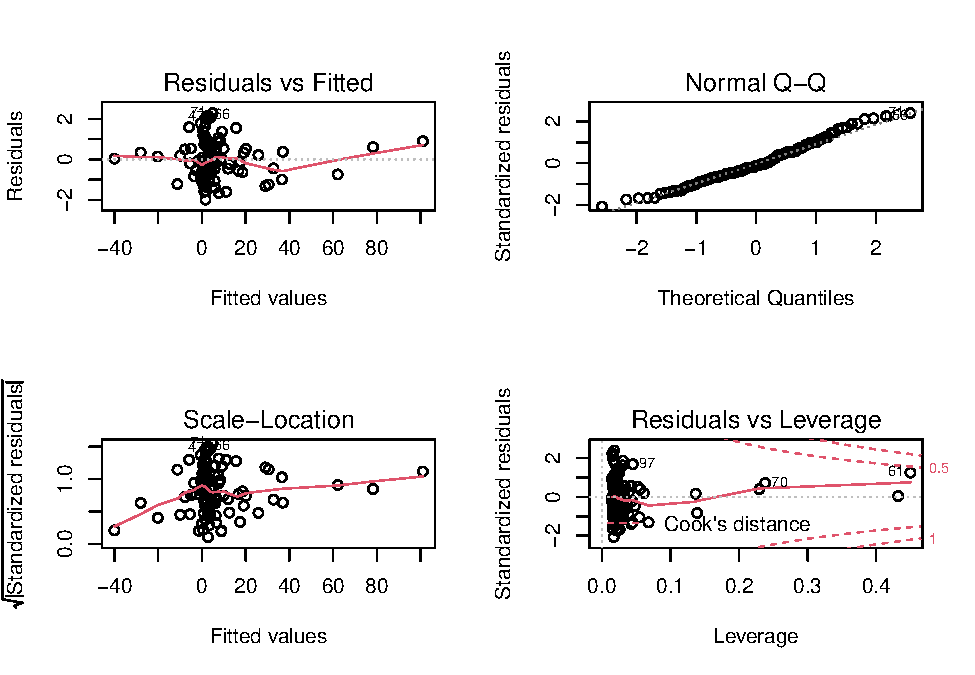
\includegraphics{math4322_fall21_hw2_files/figure-latex/unnamed-chunk-26-1.pdf}
(d) Repeat (c), using forward stepwise selection and also using
backwards stepwise selection. How does your answer compare to the
results in (c)?

\begin{Shaded}
\begin{Highlighting}[]
\FunctionTok{step}\NormalTok{(}\FunctionTok{lm}\NormalTok{(Y}\SpecialCharTok{\textasciitilde{}}\FunctionTok{poly}\NormalTok{(predictorx, }\DecValTok{10}\NormalTok{)), }\AttributeTok{direction =} \StringTok{"backward"}\NormalTok{)}
\end{Highlighting}
\end{Shaded}

\begin{verbatim}
## Start:  AIC=4.64
## Y ~ poly(predictorx, 10)
## 
##                        Df Sum of Sq     RSS    AIC
## <none>                                 84.1   4.64
## - poly(predictorx, 10) 10     28861 28944.7 568.80
\end{verbatim}

\begin{verbatim}
## 
## Call:
## lm(formula = Y ~ poly(predictorx, 10))
## 
## Coefficients:
##            (Intercept)   poly(predictorx, 10)1   poly(predictorx, 10)2  
##                 6.5842                140.2677                 59.4663  
##  poly(predictorx, 10)3   poly(predictorx, 10)4   poly(predictorx, 10)5  
##                75.1300                  1.2571                  1.4802  
##  poly(predictorx, 10)6   poly(predictorx, 10)7   poly(predictorx, 10)8  
##                 0.1190                 -0.3298                 -0.1079  
##  poly(predictorx, 10)9  poly(predictorx, 10)10  
##                -0.2958                 -0.9512
\end{verbatim}

\begin{Shaded}
\begin{Highlighting}[]
\FunctionTok{step}\NormalTok{(}\FunctionTok{lm}\NormalTok{(Y}\SpecialCharTok{\textasciitilde{}}\FunctionTok{poly}\NormalTok{(predictorx, }\DecValTok{10}\NormalTok{)), }\AttributeTok{direction =} \StringTok{"forward"}\NormalTok{)}
\end{Highlighting}
\end{Shaded}

\begin{verbatim}
## Start:  AIC=4.64
## Y ~ poly(predictorx, 10)
\end{verbatim}

\begin{verbatim}
## 
## Call:
## lm(formula = Y ~ poly(predictorx, 10))
## 
## Coefficients:
##            (Intercept)   poly(predictorx, 10)1   poly(predictorx, 10)2  
##                 6.5842                140.2677                 59.4663  
##  poly(predictorx, 10)3   poly(predictorx, 10)4   poly(predictorx, 10)5  
##                75.1300                  1.2571                  1.4802  
##  poly(predictorx, 10)6   poly(predictorx, 10)7   poly(predictorx, 10)8  
##                 0.1190                 -0.3298                 -0.1079  
##  poly(predictorx, 10)9  poly(predictorx, 10)10  
##                -0.2958                 -0.9512
\end{verbatim}

\end{document}
